\documentclass{beamer}
\usepackage[utf8]{inputenc}

\usetheme{Madrid}
\usecolortheme{default}
\usepackage{extarrows}
\usepackage{amsmath}
\usepackage{extarrows}
\usepackage{amssymb,amsfonts,amsthm}
\usepackage{txfonts}
\usepackage{tkz-euclide}
\usepackage{listings}
\usepackage{adjustbox}
\usepackage{array}
\usepackage{tabularx}
\usepackage{gvv}
\usepackage{lmodern}
\usepackage{circuitikz}
\usepackage{tikz}
\usepackage{graphicx}
\usepackage{amsmath} 

\setbeamertemplate{page number in head/foot}[totalframenumber]

\usepackage{tcolorbox}
\tcbuselibrary{minted,breakable,xparse,skins}

\definecolor{bg}{gray}{0.95}
\DeclareTCBListing{mintedbox}{O{}m!O{}}{%
  breakable=true,
  listing engine=minted,
  listing only,
  minted language=#2,
  minted style=default,
  minted options={%
    linenos,
    gobble=0,
    breaklines=true,
    breakafter=,,
    fontsize=\small,
    numbersep=8pt,
    #1},
  boxsep=0pt,
  left skip=0pt,
  right skip=0pt,
  left=25pt,
  right=0pt,
  top=3pt,
  bottom=3pt,
  arc=5pt,
  leftrule=0pt,
  rightrule=0pt,
  bottomrule=2pt,
  toprule=2pt,
  colback=bg,
  colframe=orange!70,
  enhanced,
  overlay={%
    \begin{tcbclipinterior}
    \fill[orange!20!white] (frame.south west) rectangle ([xshift=20pt]frame.north west);
    \end{tcbclipinterior}},
  #3,
}
\lstset{
    language=C,
    basicstyle=\ttfamily\small,
    keywordstyle=\color{blue},
    stringstyle=\color{orange},
    commentstyle=\color{green!60!black},
    numbers=left,
    numberstyle=\tiny\color{gray},
    breaklines=true,
    showstringspaces=false,
}
\title %optional
{12.462}


\author 
{Kartik Lahoti - EE25BTECH11032}

\begin{document}


\frame{\titlepage}
\begin{frame}{Question}
The signal $x\sbrak{n}$ shown  is convolved with itself to get $y\sbrak{n}$. The value of $y\sbrak{-1}$ is 
    \centering
    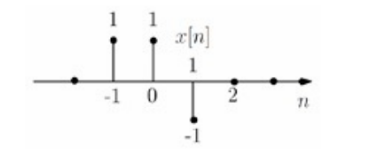
\includegraphics[width=\columnwidth, height=0.8\textheight, keepaspectratio]{../figs/q1.png}
\end{frame}

\begin{frame}{Theoretical Solution}

The Opertation 

\begin{align}
    x\sbrak{n} * x\sbrak{n} = y\sbrak{n} 
\end{align}

Can be written as 

\begin{align}
    \vec{y} = \vec{M}\vec{x}
\end{align}

Where , $\vec{M}$ is a special kind of matrix called a Toeplitz matrix formed from the signal $x\sbrak{n}$

\end{frame}

\begin{frame}{Theoretical Solution}
Given , 

\begin{align}
    \vec{x} = \myvec{x\sbrak{-1}\\x\sbrak{0}\\x\sbrak{1}} = \myvec{1\\1\\-1}. \\x\sbrak{n} = 0 , \text{ where } n \notin \cbrak{-1,0,1}
\end{align}

\begin{align}
    \vec{M} = \myvec{x\sbrak{-1}&0&0\\x\sbrak{0}&x\sbrak{-1}&0\\x\sbrak{1}&x\sbrak{0}&x\sbrak{-1}\\0&x\sbrak{1}&x\sbrak{0}\\0&0&x\sbrak{1}}
\end{align}
\end{frame}

\begin{frame}{Theoretical Solution}
\begin{align}
    \vec{y} = \vec{M}\myvec{x\sbrak{-1}\\x\sbrak{0}\\x\sbrak{1}} = \myvec{1&0&0\\1&1&0\\-1&1&1\\0&-1&1\\0&0&-1}\myvec{1\\1\\-1}
\end{align}

To find $y\sbrak{-1}$ , we perform matrix multiplication for the second row.

\begin{align}
    y\sbrak{-1} &= \myvec{1&1&0}\myvec{1\\1\\-1}\\
    &=2
\end{align}

Hence, $y\sbrak{-1}= 2$
\end{frame}


\end{document}
